\documentclass[11pt]{article}
\usepackage[letterpaper,margin=1in]{geometry}
\usepackage{amsmath,amssymb}
\usepackage{graphicx}
\usepackage{xcolor}
\usepackage{tcolorbox}
\usepackage{enumitem}
\usepackage{booktabs}
\usepackage{array}
\usepackage{hyperref}

\definecolor{tdcolor}{HTML}{2A4D6E}
\definecolor{sdcolor}{HTML}{7A3B2E}
\definecolor{boxbg}{HTML}{F4F4F0}

\tcbset{
  answerbox/.style={
    colback=boxbg, colframe=black!60, boxrule=0.5pt,
    left=8pt, right=8pt, top=6pt, bottom=6pt, arc=2pt
  }
}

\newcommand{\tdhead}[1]{{\large\bfseries\color{tdcolor} #1}}
\newcommand{\sdhead}[1]{{\large\bfseries\color{sdcolor} #1}}

\setlength{\parindent}{0pt}
\setlength{\parskip}{6pt}

\title{\bfseries Why Go to the $s$-Domain?\\[2pt]\large A Worked Comparison on a Two-Mass, Two-Spring System}
\author{}
\date{}

\begin{document}
\maketitle
\vspace{-1.5em}

The Laplace transform is usually introduced as a table of rules. What it's
\emph{for} is easy to lose: turning a differential equation into an algebra
problem. For a single spring--mass--damper, that trade barely shows --
solving the ODE directly and solving it via Laplace take about the same
amount of work. This handout uses a slightly bigger system -- two masses
coupled by two springs, no damping -- where the trade becomes obvious.

We solve the \emph{same} system, for the \emph{same} input, twice: once
entirely in the time domain, once via the $s$-domain round trip. Both
routes must agree -- and they do, exactly. What's worth watching is
\emph{how much work each route costs}, and how that cost changes as the
system gets more complicated.

\section*{The System}

Two masses $m_1=m_2=1$, two springs $k_1=k_2=1$, no friction anywhere. An
input force $u(t)$ drives $m_1$ through spring $k_1$; $m_1$ is coupled to
$m_2$ through spring $k_2$. The output is $x_2$, the position of the
second mass. The equations of motion are:
\[
\ddot x_1 + 2x_1 = u + x_2
\qquad\qquad
\ddot x_2 + x_2 = x_1
\]
We'll drive the system with a unit step, $u(t)=1$ for $t\ge 0$, starting
from rest: $x_1(0)=\dot x_1(0)=x_2(0)=\dot x_2(0)=0$.

\bigskip
\hrule
\bigskip

\tdhead{Route 1: Solve Directly in the Time Domain}

\subsection*{Step 1 -- Eliminate $x_1$}

We want a single equation in $x_2$ alone. From the second equation,
$x_1 = \ddot x_2 + x_2$. Differentiating \emph{twice} to get $\ddot x_1$:
\[
\ddot x_1 = x_2^{(4)} + \ddot x_2
\]
Substitute both into the first equation:
\[
\big(x_2^{(4)}+\ddot x_2\big) + 2\big(\ddot x_2 + x_2\big) = u + x_2
\quad\Longrightarrow\quad
x_2^{(4)} + 3\ddot x_2 + x_2 = u
\]
For our unit step ($u=1$):
\[
x_2^{(4)} + 3\ddot x_2 + x_2 = 1
\]
This already cost us two extra differentiations just to get a solvable
single-variable equation -- work that scales up fast with every extra
mass added to the chain.

\subsection*{Step 2 -- Homogeneous solution}

Characteristic equation: $r^4+3r^2+1=0$. Substitute $y=r^2$:
\[
y^2+3y+1=0 \quad\Longrightarrow\quad y = \frac{-3\pm\sqrt5}{2}
\]
Both roots are negative, so $r^2$ is negative both times: the four roots
are purely imaginary, $r=\pm i\omega_1,\ \pm i\omega_2$, with
\[
\omega_1=\sqrt{\tfrac{3-\sqrt5}{2}}\approx 0.618
\qquad\qquad
\omega_2=\sqrt{\tfrac{3+\sqrt5}{2}}\approx 1.618
\]
(No damping anywhere in the system, so no decay -- purely imaginary
poles are exactly what we should expect.) The homogeneous solution is
\[
x_{2,h}(t) = A\cos\omega_1 t + B\sin\omega_1 t + C\cos\omega_2 t + D\sin\omega_2 t
\]

\subsection*{Step 3 -- Particular solution}

Constant forcing $\Rightarrow$ try a constant $x_{2,p}=K$: all derivatives
vanish, leaving $K=1$. General solution:
\[
x_2(t) = 1 + A\cos\omega_1 t + B\sin\omega_1 t + C\cos\omega_2 t + D\sin\omega_2 t
\]

\subsection*{Step 4 -- The hidden cost: four initial conditions on $x_2$}

The physics only handed us $x_2(0)=0$ and $\dot x_2(0)=0$. A 4th-order
equation needs \emph{four}. The other two are not given -- we have to go
back to the \emph{original coupled equations} to derive them:
\[
\ddot x_2 = x_1 - x_2 \ \Longrightarrow\ \ddot x_2(0) = x_1(0)-x_2(0) = 0
\]
\[
\dddot x_2 = \dot x_1 - \dot x_2 \ \Longrightarrow\ \dddot x_2(0) = \dot x_1(0)-\dot x_2(0) = 0
\]
This step has no counterpart in the $s$-domain route -- there, ``zero
initial conditions'' is a one-line assumption and nothing more is asked
of it. Here, every extra order of the ODE means hunting down one more
derivative's worth of initial condition from the original system.

\subsection*{Step 5 -- Solve for $A,B,C,D$}

Differentiate the general solution three times and evaluate all four at
$t=0$:
\[
\begin{aligned}
x_2(0) &= 1 + A + C = 0 \\
\dot x_2(0) &= B\omega_1 + D\omega_2 = 0 \\
\ddot x_2(0) &= -A\omega_1^2 - C\omega_2^2 = 0 \\
\dddot x_2(0) &= -B\omega_1^3 - D\omega_2^3 = 0
\end{aligned}
\]
The second and fourth equations involve only $B,D$: solving them together
forces $B\omega_1(\omega_1^2-\omega_2^2)=0$, and since $\omega_1\ne\omega_2$,
\[
B = 0, \qquad D = 0
\]
The first and third equations involve only $A,C$:
\[
A+C=-1, \qquad A\omega_1^2 + C\omega_2^2 = 0
\]
Solving this $2\times 2$ system:
\[
A = \frac{-5-3\sqrt5}{10} \approx -1.1708
\qquad\qquad
C = \frac{3\sqrt5-5}{10} \approx 0.1708
\]

\subsection*{Step 6 -- Final answer}

\begin{tcolorbox}[answerbox]
\[
x_2(t) = 1 - 1.1708\cos(0.618\,t) + 0.1708\cos(1.618\,t)
\]
\end{tcolorbox}

Six steps, two of them (eliminating $x_1$, then hunting down hidden
initial conditions) pure bookkeeping that exists only because we're
working in the time domain.

\newpage
\sdhead{Route 2: The $s$-Domain Round Trip}

\subsection*{Step 1 -- Transform both equations}

Zero initial conditions turn every derivative into a power of $s$, with
\emph{no extra work}: $\mathcal L\{\ddot x\} = s^2 X(s)$, full stop --
no matter how high the order.
\[
(s^2+2)\,X_1(s) = U(s) + X_2(s)
\qquad\qquad
(s^2+1)\,X_2(s) = X_1(s)
\]

\subsection*{Step 2 -- Eliminate $X_1$ -- pure algebra}

Solve the first equation for $X_1$ and substitute into the second:
\[
X_1(s) = \frac{U(s)+X_2(s)}{s^2+2}
\qquad\Longrightarrow\qquad
(s^2+1)(s^2+2)\,X_2(s) = U(s) + X_2(s)
\]
\[
X_2(s)\Big[(s^2+1)(s^2+2) - 1\Big] = U(s)
\qquad\Longrightarrow\qquad
X_2(s)\big[s^4+3s^2+1\big] = U(s)
\]
\[
X_2(s) = \frac{U(s)}{s^4+3s^2+1}
\]
Same denominator as Route 1's characteristic polynomial -- reached with
two lines of algebra, no differentiation, no elimination-by-substitution
gymnastics.

\subsection*{Step 3 -- Plug in the input}

Unit step: $U(s) = 1/s$.
\[
X_2(s) = \frac{1}{s\,(s^4+3s^2+1)} = \frac{1}{s\,(s^2+\omega_1^2)(s^2+\omega_2^2)}
\]

\subsection*{Step 4 -- Partial fractions}

\[
X_2(s) = \frac{1}{s} + \frac{B_1 s + C_1}{s^2+\omega_1^2} + \frac{B_2 s + C_2}{s^2+\omega_2^2}
\]
Clearing denominators and matching powers of $s$ (a purely mechanical,
table-driven procedure) gives $C_1=C_2=0$ automatically, and
\[
B_1 = \frac{-5-3\sqrt5}{10} \approx -1.1708 \qquad\qquad
B_2 = \frac{3\sqrt5-5}{10} \approx 0.1708
\]
-- the \emph{exact same numbers} as $A$ and $C$ from Route 1, arrived at
by matching polynomial coefficients instead of solving a linear system
built from four derivatives.

\subsection*{Step 5 -- Inverse transform, term by term}

Using only $\mathcal L^{-1}\{1/s\}=1$ and
$\mathcal L^{-1}\{s/(s^2+\omega^2)\}=\cos\omega t$ from the table:
\[
x_2(t) = 1 + B_1\cos\omega_1 t + B_2\cos\omega_2 t
\]

\subsection*{Step 6 -- Final answer}

\begin{tcolorbox}[answerbox]
\[
x_2(t) = 1 - 1.1708\cos(0.618\,t) + 0.1708\cos(1.618\,t)
\]
\end{tcolorbox}

\emph{Identical to Route 1} -- as it must be, since both routes solve the
same equations. (For what it's worth: $0.618\ldots$ and $1.618\ldots$ are
$1/\varphi$ and $\varphi$, the golden ratio -- a fact of this particular
characteristic polynomial, $s^4+3s^2+1$, not a general feature of coupled
spring--mass systems.)

\newpage
\section*{The Comparison}

\begin{center}
\renewcommand{\arraystretch}{1.4}
\begin{tabular}{p{3.6cm} p{5.6cm} p{5.6cm}}
\toprule
& \textbf{\color{tdcolor}Time domain} & \textbf{\color{sdcolor}$s$-domain} \\
\midrule
Turning the ODEs into something solvable &
Eliminate $x_1$ by substitution, requiring two extra differentiations &
One line of algebra per equation \\
Handling initial conditions &
Must \emph{derive} $\ddot x_2(0)$, $\dddot x_2(0)$ from the original coupled system -- one extra derivation per extra order &
Built into the transform; zero I.C.'s cost nothing, nonzero I.C.'s cost one extra term per derivative \\
Finding the unknown constants &
Solve a $4\times4$ linear system built from evaluating derivatives at $t=0$ &
Match polynomial coefficients (partial fractions) -- no derivatives involved \\
Scaling to a 3-mass system, or adding damping &
Every step above gets harder: more differentiations, more hidden I.C.'s to hunt down, a bigger linear system &
Same three steps (transform $\to$ algebra $\to$ partial fractions) -- just bigger polynomials \\
\bottomrule
\end{tabular}
\end{center}

\bigskip
\textbf{The point isn't that the $s$-domain is a trick.} It's that
differentiation becomes multiplication by $s$, and initial conditions
get absorbed into the transform itself instead of requiring a fresh
derivation every time the model gets one order bigger. For a single
spring--mass--damper that trade is barely worth noticing. For a coupled,
higher-order system, it's the difference between a page of algebra and a
page of calculus.

\bigskip
\begin{center}
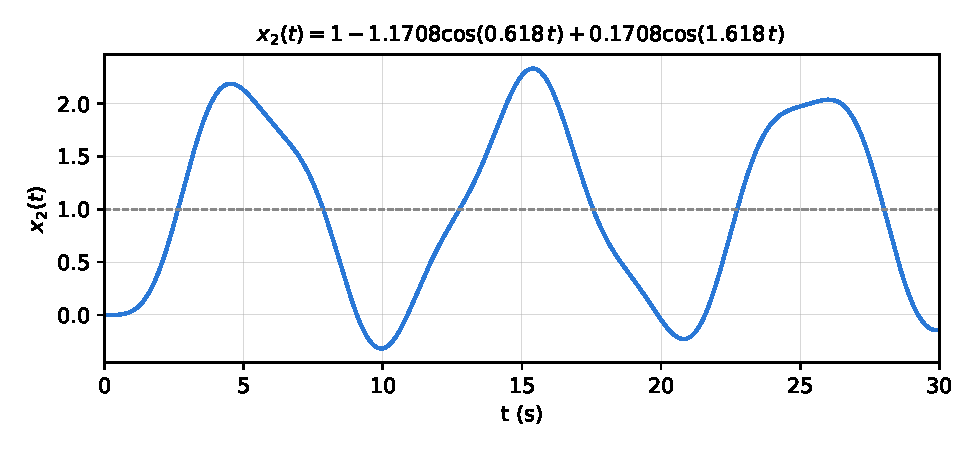
\includegraphics[width=0.85\linewidth]{x2_response.pdf}
\end{center}
\begin{center}
\small Both routes agree exactly: an undamped system oscillates forever
around its steady-state value of $1$, beating between the two natural
frequencies $\omega_1\approx0.618$ and $\omega_2\approx1.618$ rad/s.
\end{center}

\end{document}
